%!TEX root=../oi-magistr-spolecne.tex
\section[KO - Scheduling]{Rozvrhování na jednom procesoru a na paralelních procesorech. Rozvrhování projektu s časovými omezeními. Programování s omezujícími podmínkami.}


\subsection{Rozvrhování}
Rozvhrování obecně je přiřazení úloh zdrojům v čase. Na vstupu je typicky množina úloh k rozvržení, každá z nich má své parametry (délka zpracování, termín dokončení apod.). Dále jsou v problému zdroje (typicky nějaké stroje nebo lidská síla), ty jsou určeny počtem (kapacitou) a každý jednotka zdroje může mít v čase přiřazen max. jednu úlohu. Cílem je rozvrhnout (přiřadit) všechny úlohy v čase při dodržení všech omezení. Přičemž rozvrh by měl být v nějakém smyslu optimální - to určuje kriteriální funkce (např. minimální délka rozvrhu).

\paragraph{Některé parametry:}
\begin{itemize}[itemsep=0px]
\item \textbf{release time} $r_j$ - čas, kdy úlohu lze nejdřív rozvrhnout
\item \textbf{process time} $p_j$ - doba zpracování
\item \textbf{due date} $d_j$ - termín, kdy by úloha měla být dokončena
\item \textbf{deadline} $\widetilde{d_j}$ - termín, kdy úloha musí být dokončena
\item \textbf{start čas} $s_j$, \textbf{čas dokončení} $c_j$
\item \textbf{čas čekání} $w_j = s_j - r_j$
\item \textbf{lateness} $L_j$ - rozdíl doby dokončení od due datu $c_j - d_j$
\item \textbf{tardiness} $D_j$ - zpoždění = doba dokončení po due datu $\max\{c_j - d_j,0\}$
\end{itemize}

\begin{figure}[h]
    \begin{center}
        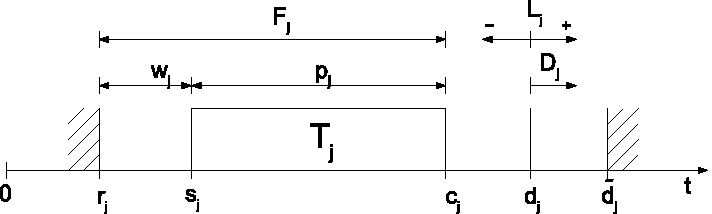
\includegraphics[width=100mm]{10/images/scheduling-params}
    \end{center}
\end{figure}

\paragraph{Notace rozvrhovacích problémů:} $\alpha | \beta | \gamma$ (příklad: $1|r_j,d_j|C_{max}$)
\begin{itemize}
\item $\alpha$ - popisuje zdroje, jejich počet a typ (paralelní,uniformní, unrelated, job shop, atd)
\item $\beta$ - popisuje omezení jobů (precedence, preempce, due dates, deadlines, process times)
\item $\gamma$ - popisuje kritérium rozvrhu - délka rozvrhu ($C_{max}$), lateness, tardiness
\end{itemize}

\subsection{Rozvrhování na jednom procesoru}
Mnoho \uv{easy} problémů ($1|prec|C_{max}$, $1||C_{max}$, $1|r_j|C_{max}$, $1|\widetilde{d_j}|C_{max}$) - jen seřadíme úlohy např. podle $\widetilde{d_j}$. Kombinace $1|r_j,\widetilde{d_j}|C_{max}$ už není tak jednoduchá (NP-hard).

\paragraph{Bratleyův B\&B alg} Řeší \textbf{$1|r_j,\widetilde{d_j}|C_{max}$} které je \textbf{NP-hard}. Klasický branch\&bound, když překročíme deadline, můžeme odříznout i bratry. Když narazíme na řešení, zkusíme test optimality - má první úloha nejmenší release time? Jestli jo, break jinak jedeme dál.

\begin{figure}[h]
    \begin{center}
        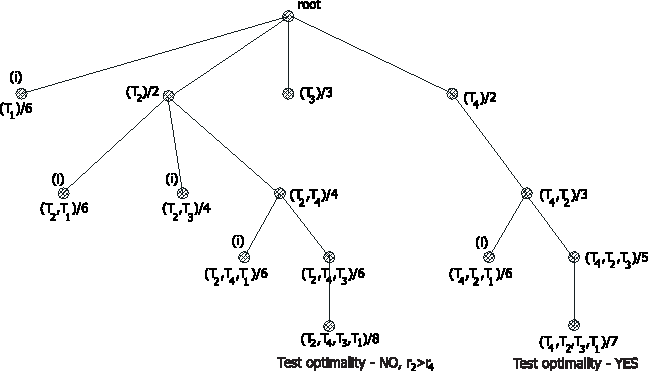
\includegraphics[width=130mm]{10/images/bratley}
    \end{center}
    \caption{Bratleyův alg pro: $r=[4,1,1,0], p=[2,1,2,2], \widetilde{d}=[8,5,6,4]$}
\end{figure}

$1|prec|\sum wC$ se řeší branch\&bound s LP. Definujeme problém jako LP (rozhodovací proměnná $x_{ij} = 1 $ iff úloha $i$ je předchůdce $j$), což nám dá hodnotu zbylých úloh. Ořezáváme, pokud řešení + zbylé úlohy > dosud nejlepší řešení.

\subsection{Rozvrhování na paralelních procesorech}
\paragraph{McNaughton $O(n)$} Řeší $P|pmtn|C_{max}$. Spočítám si $C_{max}$ jako maximum ze součtu časů/počet procesorů a času nejdelšího úkolu:

$$C^{*}_{max} = \max \{{{1} \over {R}} \sum^{n}_{i = 1} p_{i}, \max_{i = 1, \cdots, n} p_{i} \}$$

Nyní, když je již známá délka rozvrhu, může algoritmus přistoupit k samotnému plánování. Algoritmus iteruje postupně přes všechny úkoly a vyplňuje matici od levého horního rohu po řádcích. První úkol umístí do levého horního rohu, druhý úkol těsně za něj a tak dále. V okamžiku, kdy se některý z úkolů již nevejde celý na jeden řádek (zdroj), tak jej algoritmus přeruší (nechá na k-tém zdroji vykonat pouze koncovou část úkolu), a jeho první část rovrhne na zdroj následující.

\begin{itemize}
\item $P2||C_{max}$ NP-hard - lze převést z 2-partition problému.
\item $P|pmtn,r,d|C_{max}$ jde formulovat jako úlohu maximálního toku: Udělám si intervaly pro všechny release timy a deadliny. Každý interval bude jeden vrchol. Každá úloha bude vrchol. Od zdroje k úlohám budou mít hrany hodnotu doby trvání. Od úloh do intervalových vrcholů budou mít hrany kapacitu velikosti intervalu. Od vrcholu do zdroje je kapacita velikost intervalu * počet procesorů.
\end{itemize}

\paragraph{List Scheduling (LS) $P|prec|C_{max}$} Aproximační alg. Nejdřív dám do listu úlohy bez předchůdců. Postupně přiřazuju z listu na procesory a když to někde doběhne, dám tam další a na konec listu dám následovníky té co doběhnula. Aproximační faktor $r_{LS} = 2 - \frac{1}{R}$ (R je počet zdrojů).

\textbf{Longest processing time first (LPT) $P||C_{max}$} Vylepšení pro LS v podobě vhodného řazení úloh. Funguje stejně jako LS ale řadím list podle processing timu. Aprox faktor $r_{LPT} = \frac{4}{3} - \frac{1}{3R}$. Tento problém se dá řešit ještě pomocí pseudopolynomiálního dynamického programování Rothkopf (R-rozměrné pole).

\textbf{Rothkopf} řeší dynamickým programováním pseudopolynomiálně P||Cmax. Mám tabulky časů pro každý procesor, počet rozměrů stejně jako procesorů a zapisuju tam všechny možnosti. Na konci minimalizuju rozdíl časů na jednotlivých procesorech.

\paragraph{Úrovňový algoritmus $P|pmtn,prec|C_{max}$} řeší $P|pmtn,prec|C_{max}$ v $(n^2)$. Nejdřív ohodnotím graf následností úrovněmi.

Algoritmus nejprve zkonstruuje graf závislostí, v němž jsou úkoly vyjádřené pomocí uzlů a relace následností pomocí orientovaných hran (hrana vede vždy z předka do následníka). Dále algoritmus ohodnotí všechny uzly dle následujícího schématu (S(x) značí všechny následníky uzlu x):

$$level(j) = \max_{s \in S(j)}\{level(s)\} + p_J$$

Úroveň se počítá jako délka zpracování + maximální úroveň z následníků. Proto to je vhodné počítat zprava. Samotné rozvrhování probíhá v časových kvantech. Na každý zdroj je umístěn úkol s nejvyšší úrovní. Po obsazení všech zdrojů je spuštěno zpracování úkolů na zdrojích na časové kvantum $T$, které odpovídá času do zpracování nejkratšího z úkolů. Po vykonání tohoto kvanta je zpracovaný úkol odstraněn a u částečně zpracovaných úkolů je snížena jejich úroveň o $T$ (úroveň se skládá také z délky úkolu a ta je nyní kratší). Na zdroje jsou znovu umístěny úkoly s nejvyšší úrovní (jejichž všichni předci již byli zpracováni), což ale nemusí být nutně ty, které byly částečně zpracovány v minulé iteraci. Algoritmus terminuje v okamžiku zpracování všech úkolů.

\begin{figure}[h]
    \begin{center}
        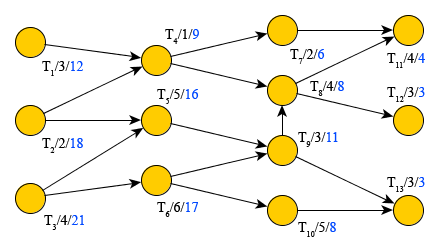
\includegraphics[width=80mm]{10/images/level-alg}
        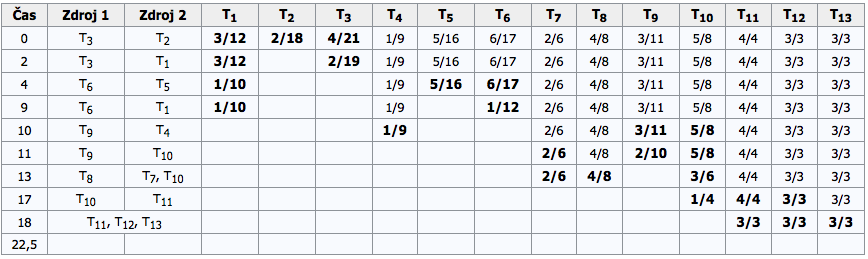
\includegraphics[width=130mm]{10/images/level-alg-tab}
    \end{center}
    \vspace{-5px}
    \caption{Úrovňový algoritmus}
    \vspace{-5px}
\end{figure}


\subsection{Rozvrhování projektu (Project scheduling)}
Je scheduling s temporálními omezeními. $PS|temp|C_{max}$ - NP-obtížný problém. Temporální omezení jsou relace následností s váhami na hranách. Když váha = $p_j$ předchozí, můžu začít když ta předchozí skončí. Když váha > $p_j$, musím čekat. Když 0 < váha < $p_j$, musím začít během vykonávání na jiném procesoru. Řeší se pomocí ILP - binární nebo celočíselná formulace.

\subsection{Programování s omezujícími podmínkami (Constraint Programming)}
Je podobný jako ILP, ale můžeme definovat víc druhů podmínek (ILP jenom nerovnice, CSP libovolné relace). Kromě \textbf{omezení} se definují domény \textbf{pro} každou \textbf{proměnnou} - např. \textbf{sudoku} 1-9.

Postup: nejdřív udělám úvodní propagaci - aplikuji podmínky na obor hodnot. Potom jedu b\&b, postupně zkouším jednotlivé data a propaguji podmínky. Až se dostanu k nějakému řešení. Hranová konzistence znamená, že hrana s daným řešením splňuje všechna omezení.

Jeden z algoritmů pro řešení je AC-3. Při \textbf{AC3} si udržujeme \textbf{frontu hran}, které je potřeba \textbf{revidovat}. Na začátku jsou tam všechny hrany a postupně je odebíráme. Pozor, revizí nějaké hrany se může znevalidnit už validovaná hrana. Algoritmus běží, dokud nejsou všechny hrany konzistentní. Vždy reviduju přechody nejdříve v jednom směru a pak v druhém. pokud se mi změní doména (odeberu číslo), tka musím opět dát do fronty tu hranu, které se doména týká.

\begin{figure}[h]
    \begin{center}
        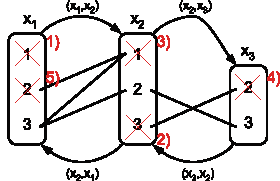
\includegraphics[width=60mm]{10/images/ac3}
    \end{center}
    \vspace{-10px}
    \caption{AC-3: $x_1 > x_2, x_2 \neq x_3, x_2+x_3 > 4; D_1 = \{1,2,3\}, D_2 = \{1,2,3\}, D_3 = \{2,3\}$}
\end{figure}
